\chapter{转发分析}
\label{ch6}

\section{引言}
\label{ch6_intro}
信息传播在市场营销以及选举策略等应用场景发挥着很大的作用,因为通过信息传播可以触发大量的人参与并逐步层叠扩展到更多的人。信息传播的研究引起了很多研究者的关注,尤其是在线的社交网络的研究者,他们对信息传播提出了一些通用的模型,用于帮助模拟信息流动(information flow)\upcite{Goldenberg2001,Kempe2003}以及探测信息级联(information cascades)的爆发\upcite{Cheng2014}。可是他们常常都是将用户看作是网络中单一的节点,忽略了用户在信息传播过程中的自主性。作为Web2.0时代的信息消费者和生产者,每个用户都可以在社交媒体上发帖表明自己的兴趣和观点,选择信息阅读和传播。在社交网络上一条信息能否获得广泛传播依赖于“口碑相传(word of mouth)”效应,该效应会引发用户的传播行为。随着自然语言处理(Natural Language Processing)和数据挖掘(data mining)技术的发展,社交媒体上用户的意图可以使用他们产生的数据对用户进行建模来分析。本章中,我们关注一个有趣的问题:“口碑相传”效应机制问题,也就是给定某个特定用户的一条新微博,我们想要预测在所有收到该微博的所有用户中谁最有可能参与到该条信息的后续传播中去。作为一个典型的场景,我们用在Twitter中的一个异构网络来说明这个问题,如图~\ref{fig6-0}所示,网络中Tony和他的网络中的朋友讨论了两个话题:“苹果手机(Iphone)"以及电影"冰雪奇缘(Frozen)",现在Tony发了一条有关电影“冰雪奇缘”的新微博,我们想去发现他的朋友中谁会转发这条微博进行传播。

\begin{figure}[htb]
\centering
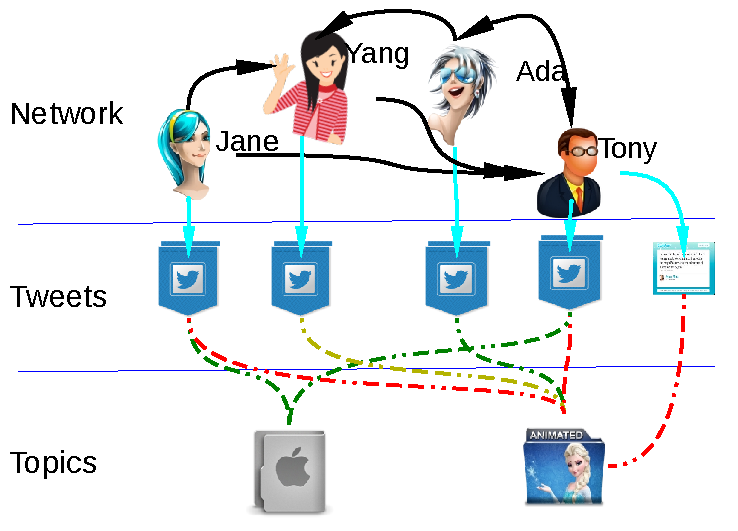
\includegraphics[height=170pt]{6-0.pdf}
\caption{问题图示}
\label{fig6-0}
\end{figure}
\footnotetext{每个用户的观点用不同颜色表示,“红色”当标正面观点,“绿色”代表负面观点,“黄色”代表中性观点。}

不同社交网络平台上的信息传播行为是不一样的,本章我们主要研究Twitter上的转发行为。因为庞大的用户群以及信息的爆炸式增长,Twitter在互联网上信息传播中扮演着重要角色,尽管微博长度上受到限制,但是Twitter为用户提供的转发按钮为信息的快速传播提供了前所未有的机制。据统计Twitter上的微博超过四分之一是转发别人的\upcite{yang2010understanding},因此如果能够理解了转发行为是如何发生的也就能很好的解释Twitter上的信息传播。

作为信息传播的参与者,用户很自然地会在相互通信交互中表达出自己感兴趣的话题并发表自己的观点。在心理学的研究中证实人的主观能动性(subjective initiative)本质决定了人的主观性会影响其行为\upcite{Moore2008},同样根据偏颇吸收(Biased Assimilation)理论,人总是趋向于选择和传播跟自己偏执观点(biased opinions)相似的信息\upcite{Hyman2000}。因此能够全面掌握用户的主观性是研究用户参与信息传播意图的一个很重要的方面。针对转发行为的前期研究已经发展出了一些方法和模型用于找到影响转发的因素\upcite{Macskassy2011,Feng2013}。然而据我们所知,还没与研究关注到用户转发行为背后的主观动机。就Twitter的口碑效应来说,转发意味着包括接受消息,评估内容以及衡量时候转发三个环节的一个完整过程,其中最重要的就是评估消息中是否有价值的信息值得和朋友分享。因此对用户的主观动机进行建模会为转发行为分析提供重要的研究视角。直觉上,依据“物以类聚(like attracts like)”原则,具有主观性的用户更趋向于转发那些能够迎合他口味(观点)的信息。就我们在图~\ref{fig6-0}中的例子来说,用户对两个话题所持观点已经在他们之前发布的微博中表达了,Tony和Jane对电影“冰雪奇缘”持正面肯定观点,而Ada持负面观点,Yang持中性观点。如果Tony新发布的是对冰雪奇缘正面肯定的微博,Jane是最有可能转发这条微博的就很容易理解了。因此用户的主观性是如何影响其转发行为的是本章的关注点。

为了研究主观性和转发行为的关系,有两个问题需要回答:(1)怎样准确对用户的主观性进行建模?(2)怎么样从主观性上有效度量用户认为微博传播的值得性?
回答这两个问题不是一件很容易的事,其中上一章我们已经提出了使用主观模型来解决社交媒体上用户观点集成问题,本章我们将继续使用主管模型的概念,提出一个更加通用的框架,并就主管模型提出一个全新的相似性计算方法来度量传播的值得性,而且就影响转发行为的因素,我们会结合主观相似性度量来分析三个最有可能引起转发行为的因素。

\section{相关工作}
\label{ch6_relatedwork}
在微博转发行为分析方面,很多工作已经在转发行为特征、查找提高微博转发性的因素以及设计能估计转发概率的模型方面展开研究。Suh等~\upcite{suh2010want}通过研究发现带有网络连接URL以及hashtag标记的微博更有可能被转发。Macskassy和Michelson~\upcite{Macskassy2011}发现从微博内容中推到得出的模型能够解释大多数的转发行为。Comarela等\upcite{comarela2012understanding}发现对微博作者的先前反应,微博作者发帖频率,微博内容的新鲜程度以及微博的长度会影响关注者的转发可能性。Starbird和Palen~\upcite{starbird2012will}特别针对危机发生时的微博信息转发机制进行了研究,发现带有跟带有危机话题关键词的微博更有可能被转发。Osborne和Lavrenko~\upcite{petrovic2011rt}通过引入一些有用特征,比如微博的新颖性和作者被加入朋友列表的次数,来使用被动主动算法(passive aggressive algorithm)训练模型预测转发行为。Jenders等~\upcite{jenders2013analyzing}从微博及其作者的网络结构、信息内容以及情感方面分析了一些“显式”和“隐式”的影响转发的特征。Naveed等~\upcite{NaveedGKC2011,naveed2011searching}
引入了微博的趣味性指标,并使用一些比如表情符、情感以及话题等特征对其进行量化来预测一条微博被转发的可能性。Feng和Wang~\upcite{feng2013retweet}构建了一个图模型并将微博以及用户的所有信息源结合进图的节点和边,并提出了一个特征敏感的因子分解模型(factorization model)对微博依据被转发的可能概率进行重排序。Pfitzner等~\upcite{Pfitzner2012}提出了一种叫做情感分歧(emotional divergence)指标来评价微博被转发的可能性,并研究证实了高情感分歧值的微博会有更高五倍的机会被转发。

总体来说,上述所有工作主要是回答“某条微博会否被某些用户转发”这样一个问题,但是他们还不能回答“从一个信息消费者角度来看的某条微博是否值得用户采用转发行为进行信息传播”这样的问题,本章中我们会结合上章提出的主观模型从用户的兴趣和观点角度就用户的主观动机来分析转发行为。
\section{基于主观模型的转发分析}
为了研究用户转发行为的主观动机,首先需要了解用户的主观性,也就是能清楚用户喜欢什么和不喜欢什么,也就是用户感兴趣的话题和用户对话题所持的观点,这就是上章我们为用户所建立主观模型的作用。随着社交媒体普及率越来越高,社交媒体上带有用户主观性信息的用户产生内容(UGC)也越来越多,自然语言处理领域的观点挖掘(opinion mining)\upcite{Liu2012}研究开始通过计算方式自动对用户的观点信息进行建模。并且也出现了一些基于方面(aspect-based)情感分析或话题情感模型(topic-sentiment model)\upcite{Lek2013,Mei2007}将针对话题的观点投射为二值极性,评价等级或情绪类型等某一个单一的情感值,但是这些模型因为这种观点简单的表示形式而使得其作用受到限制。因此在主观模型中,我们通过将话题和观点结合为一个模型并将话题和观点使用新的表示形式(在话题空间和情感空间的分布)来对用户的主观性进行建模。

\subsection{主观模型}
\label{subjectivemodel}
在Twitter上,用户一般是对多个不同话题感兴趣,比如图~\ref{fig6-0}中的例子中Tony和Jane都对苹果手机话题和冰雪奇缘电影刚兴趣并表达了自己的观点。一般来讲,用户对话题的兴趣度会随着话题的不同而不同,而且,即便对同一个感兴趣话题,当一个用户其其不同的方面(aspects)发表微博表达的观点也不是完全一样的,因此我们认为对用户的主观性进行建模时:
\begin{itemize}
\item 每一个用户$ u $都对应着一个在话题空间$ T $的$ |T| $维的话题分布$ W_{u}=\{w_u(t)\}|W_u \in R^{|T|},\sum_{t}w_{u}(t)=1 $,其中$ w_{u}(t) $表示用户在话题$ t $上的兴趣度。
\item 用户$ u $对话题$ t $的观点应该表示为一个在情感空间$ S $的$ |S| $维的情感分布$ O_t=\{d_{u,t}(s)| O_t \in R^{|S|}, \sum_{s}d_{u,t}(s)=1\}$,其中$ d_{u,t}(s) $表示用户观点中带有情感值$ s $的可能性。
\end{itemize}

从技术角度来讲,我们提出主观模型的目标就是设计一个通用的框架能够从社交媒体用户产生的数据中同时学习到用户兴趣(对应的话题分布)和观点(对应的观点分布),以此为基础进行用户一些在线行为的分析,本章中我们主要研究用户的转发行为。之所以说我们提出的主观模型是通用的,因为它不但将用户的兴趣和观点融进一个整体框架,更重要的是,在主观模型中观点表示为一个在可扩展的情感空间上的概率分布。这个情感空间既可以是表示情感正负极性的二值空间,又可以是连续值表示的情感强度空间,或是离散值表示的情绪类型空间,因此可以覆盖所有的观点表示形式。图~\ref{fig6-1}是一个在$ [0,100] $话题空间和$ [0,8] $情感强度空间主观模型的可视化示例。

\begin{figure}[htp]
\centering
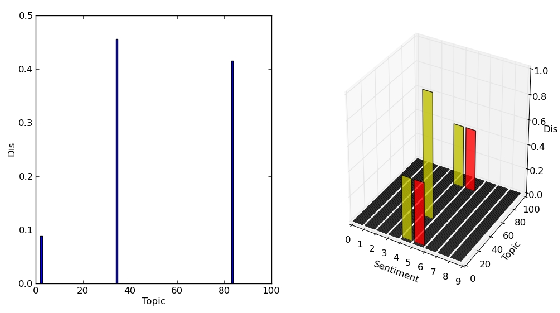
\includegraphics[height=170pt]{6-1.pdf}
\caption{可视化主观模型示例}
\label{fig6-1}
\end{figure}
左侧图中表示用户在话题2,32和83上的兴趣度:$$ (  w_{u,2}=0.08,w_{u,32}=0.48, w_{u,83}=0.44)  $$
右侧图中表示在每个话题上的观点分布:
$$ O_{2}=( d_{u,2,4} =0.5, d_{u,2,5} =0.5)$$
$$O_{32}=(d_{u,32,4}=1.0) $$ $$O_{83}=( d_{u,83,4}=0.5, d_{u,83,5}=0.5 )$$

在构建主观模型时,我们的框架是将话题分析和观点分析分开进行的。具体点来讲,首先使用的是用户层面(user-level)的LDA话题模型从用户所有的微博$M_u$中训练一个全局话题模型$ TM=(\theta,\phi) $,其中$ \theta $表示用户在话题空间$ T $的兴趣度分布,$ \phi $表示话题在词表上的分布。由于微博比较短小,通常认为每条微博谈论的是一个话题,因此我们可以根据全局话题模型计算微博$ t $从话题模型中产生的概率值为$ t $指定一个最有可能的话题:

\begin{equation}
\label{twtopic}
z_{t} = \arg \max_{k}\prod_{w \in t} P(w|\phi_{k})
\end{equation}
然后就可以将用户$ u $所有谈论同一话题的微博数进行归一化后获得用户$ u $在话题上的兴趣度:

\begin{equation}
w_{u,k}=\dfrac{|\{ t: t \in M_{u} \wedge z_{t}=k\}|}{|M_{u}|}
\end{equation}

关于观点分布,正如我们在图~\ref{fig6-0}中的例子看到,Tony和Jane总体上都是对电影“冰雪奇缘”持正面观点,但是他们有可能是因为不同的原因而喜欢这部电影的。Jane可能非常喜欢电影浪漫的故事情节,但是对它的动画画面稍微有点失望;而Tony喜欢这部电影可能是因为被这部电影的动画技术所折服,却不喜欢它略显幼稚的公主王子题材。之前的情感分析研究主要是将观点通过计算得出某一个单一值,尤其是正负极性二值为主,并不区分针对话题的每个观点在不同方面的具体情感,也无法计算观点的大小顺序,比如那个用户更喜欢电影些。因此在主观模型中,我们将观点表示为在情感空间$ S $的一个分布用以更精确的表示和区分观点。假设微博$ t $通过情感分析得出其在情感空间的情感值为$ s_t $,用户在某一话题$ k $上的观点分布可以通过将其所有谈论该话题微博在每一个情感值上的数目归一化处理后获得:

\begin{eqnarray}
O_k &= & \{ d_{u,k,s}|s \in S \} \nonumber \\
  &=& \{ \dfrac{|t:t \in M_u \wedge z_t=k \wedge s_t=s|}{|M_u|}|s \in S\}
\end{eqnarray}

\subsection{主观相似性}
\label{similarity}

得到用户的主观模型后,需要定义一个相似性度量方法来计算用户之间或用户与微博之间主观性上的距离,以量化“物以类据(like attracts like)”效应。首先我们定义在同一话题上观点的相似性计算方法。
 
\subsubsection{观点相似性}
\label{opsim}

在主观模型中观点是定义在情感空间上的分布,其每一维都代表着在对应情感值上的情感比重。实际上,为了区分观点,情感空间中的情感值并不是独立的,情感值之间有一定的顺序和大小来表示情感的强度。比如情感值为8的观点比情感值为5的观点持更正面的观点。因此常用的一些计算分布相似性的方法,比余弦相似性(cosine similarity)以及KL距离(KL-divergence),对于主观模型中观点分布相似性的计算就不适合了。如表~\ref{tab6-1}所示,假设在一个$ S=[0,8 ] $情感空间中表示的三个观点:观点$ O_{k}^{1} $是最负面(100\%分布在情感值0上。),观点$ O_{k}^{2} $是正面的(50\%分布在情感值6,50\%分布在情感值7上。),观点$ O_{k}^{3} $最正面(100\%分布在情感值8上)。

\begin{table}[htb]
%\scriptsize
\centering
\caption{观点相似性示例}
\label{tab6-1}
\begin{tabular}{|l|l|l|l|l|l|l|l|l|l|}
\hline
 & 0 & 1& 2 & 3 & 4 & 5 & 6 & 7 & 8 \\
\hline
$O_{k}^{1}$ & 1.0 & 0.0 & 0.0 & 0.0 & 0.0 & 0.0 & 0.0 & 0.0 & 0.0 \\
\hline
$O_{k}^{2}$ & 0.0 & 0.0 & 0.0 & 0.0 & 0.0 & 0.0 & 0.5 & 0.5 & 0.0 \\
\hline
$O_{k}^{3}$ & 0.0 & 0.0 & 0.0 & 0.0 & 0.0 & 0.0 & 0.0 & 0.0 & 1.0 \\
\hline
\end{tabular}
\end{table} 

假设使用常规的分布的相似性计算方法余弦相似性,就会发现三个观点之间的相似性都是0,因而出现了相似性计算方法失效,这是与事实不相符的,因为观点$ O_{k}^{2} $与观点$ O_{k}^{3} $比观点$ O_{k}^{1} $与观点$ O_{k}^{3} $更相似,它们都是持正面观点。因此观点的相似性计算不能简单将观点视为一般的概率分布来计算,或者只是观点空间的一个距离值。为了准确计算观点之间的相似性,我们将观点在情感空间的距离和分布上的相似性结合起来,提出了如下的计算观点$O_{k}^{u},O_{k}^{v} $之间相似性方法:

\begin{equation}
\label{opinionsim}
Sim(O_{k}^{u},O_{k}^{v})=\dfrac{|S|-|\sum_{i=0}^{|S|}d_{i}^{u}v_{i}-\sum_{i=0}^{|S|}d_{i}^{v}v_{i}|}{|S|}
\end{equation}
其中$ d_{i} $是第$ i^{th} $维的情感分布,$ v_{i} $是相应的情感值。

使用方法~\ref{opinionsim}计算表~\ref{tab6-1}中观点之间相似性为:
$$ Sim(O_{k}^{1},O_{k}^{3})=0 $$ $$ Sim(O_{k}^{2},O_{k}^{3})=6/8$$ $$ Sim(O_{k}^{1},O_{k}^{2})=2/8 $$。
这与我们对观点相似性的直觉理解是一致的。

\subsubsection{主观相似性}
在主观模型中,用户感兴趣的话题表示为在话题空间$ T $上不同话题的兴趣度分布,因此两个主观模型$SM_u$和$SM_v$之间的主观相似性可以将话题上的权重与对应的观点分布相似性结合起来进行集成计算:

\begin{equation}
\label{subsim}
Sim(SM_{u},SM_{v})=\sum_{k=1}^{|T_{u,v}|}\theta_{u}(k)\* Sim(O_{k}^{u},O_{k}^{v})
\end{equation}
其中$ T_{u,v} $表示两个用户之间的共同话题,可以通过对他们之间感兴趣话题的交集来获得;$ \theta_{u}(k) $代表用户$ u $在话题$ k $上的兴趣度权重。

值得注意的是,当我们测量用户$ u $在主观性上与用户$ v $有多相似性时,话题权重我们使用的是用户$ u $的话题权重,因此这个主观相似性度量方法是不对称的。之所以这么做,我们的直觉是因为用户的主观性是个人的内在感觉,因此对于另一个用户与自己主观想法上有多相似也是一个单向的感知,无需对称性的考虑。因此在度量主观相似性时,$ Sim(SM_u,SM_v)\neq Sim(SM_v,SM_u)$。

\subsection{转发行为分析}
\label{retweet}
用户的转发行为收到多种因素的影响,但是从用户的角度来讲,三种情形下会引发用户的转发:

\begin{enumerate}
\item 微博的内容对用户具有吸引力,因此用户的转发行为是根据自己的主观判断引发的;
\item 微博是由关系密切的好朋友发出的,因此用户的转发行为是因为社交需要;
\item 微薄内容是突发新闻或有趣段子而具有流行性,因此用户的转发行为是趋同需求(conformity needs)\upcite{Cialdini2004}的结果。
\end{enumerate}
这些情形是用户转发行为的不同原因,从主观动机角度分析,我们使用三个主观相似性来量化这三个因素进行转发行为的分析。

在以下的分析中,对于一条微博$ t $,假设$ F $表示该微博作者$ u_{a} $的关注者,当作者$ u_{a} $发布微博$ t $后,所有用户$ F $都会看到$ t $,至于哪个用户会转发$ t $,我们需要分析其主观动机。对于每一个关注者$ f \in F $,可以定义一个四元组$ <f, u_{a}, t, r_{f}>  $,其中$ r_{f} $是一个二值标签用以表示微博$ t $是否会被用户$ f $转发,需要我们通过分析进行预测。

\subsubsection{吸引力度量}
一般来讲,用户根据自己的主观判断,看到一个有吸引力的微博就会转发。因此我们可以通过计算微博$ t $与微博关注者$ f $之间的主观相似性来定量地度量这种吸引力。对于一条微博,它所讨论的话题$ z_t $可以使用公式~\ref{twtopic}指定,对其进行情感分析可以得到情感值$ s_t $,因此微博也能够使用主观模型进行建模,它的话题分布和观点分布都是一个100\%的单一分布。于是微博$t$对于用户$f$的吸引力就可以使用我们定义的主观相似性计算方法~\ref{subsim}进行度量:
\begin{equation}
Sim(f,t)=\theta_{f}(z_t)\* Sim(O_{z_t}^{f},O_{z_t}^{t})
\end{equation}

\subsubsection{社交性度量}
这种情形下,转发行为是基于用户的社交交互需要。由于微博是由志同道合(like-minded)的好朋友发的,转发行为是因为友谊触发而不一定是微博内容。这种情况下可以通过计算用户$ f $与微博作者$ u_a $之间的主观相似性来度量二者之间友谊的亲密程度:

\begin{equation}
Sim(f,u_a)=\sum_{k=1}^{|T_{u,v}|}\theta_{f}(k)\* Sim(O_{k}^{f},O_{k}^{u_a})
\end{equation}
同时也应该考虑到,不同类型的朋友对用户$ f $的影响力(influence)是不同的,比如用户$ f $可能会关注很多人,但是可能只会与少数几个互动频繁(转发等互动)。而且用户$ f $并不是对朋友的每条微博都感兴趣,例如在图~\ref{fig6-0}中的例子中,Jane可能会对Tony所发的关于电影“冰雪奇缘”的微博,但是对他的关于苹果手机微博不感兴趣。因此我们对用户之间的主观相似性$ Sim(f,u_a) $附加一个权重以反映不同类型朋友对用户$ f $的影响力,该权重有四部分因子组合而成。

\paragraph{专家指数因子(Expert Factor) $ w_E(u_a) $:} 
该因子代表着微博作者$ u_a $在微博接收朋友圈中相对的专家指数,专家指数越高的用户就会对其他用户有更多的影响力。本章中我们简单的根据用户$ u_a $的发帖数量在所有朋友圈中发帖总数的比例来计算专家指数。
\begin{equation}
w_E(u_a)=|M_{u_a}|/|\{M_u|u \in u_a \cup F \}|
\end{equation}

\paragraph{领导力因子(Leadership Factor) $ w_L(u_a) $:} 
我们将用户的领导力为该用户拥有的粉丝(followers)数。因此领导力因子可以通过归一化计算为:
\begin{equation}
w_L(u_a)=\log (|F|)/\log(\max)
\end{equation}
其中$ \max $是Twitter中用户的最大流行度(maximum popularity)\footnote{\url{http://twittercounter.com/pages/100}}。

\paragraph{相似性因子(Similarity Factor) $ w_S(u_a,f) $:} 
用户$ u_a $和$ f $之间的兴趣的相似性可以通过他们主观模型中话题分布之间的反KL距离(inverse KL-divergence)来度量:
\begin{equation}
w_S(u_a,f)= 1/KL(\theta_{u_a},\theta_f)
\end{equation}

\paragraph{交互因子(Interaction Factor) $ w_I(u_a,f) $:} 
用户$ u_a $和$ f $之间的交互数量$ Interation_{u_a,f} $包括他们之间的对话,相互之间的提及以及相互之间的转发等。该因子可以通过将$Interation_{u_a,f}$用用户$ u_a $和$ f $所有的微博数目归一化计算获得:
\begin{equation}
w_I(u_a,f)=|Interation_{u_a,f}| /|\{ M_{u_a}, M_f \}|
\end{equation}

总体上,将以上四个因子组合后可以得到影响权重:
\begin{equation}
\begin{split}
w_{u_a,f}= \lambda_1*w_E(u_a)+\lambda_2*w_L(u_a)+
  \lambda_3*w_S(u_a,f)+\lambda_4*w_I(u_a,f)
\end{split}
\end{equation}
其中$ \lambda_i $是一个可选权重向量以反映不同因子的影响,并且$ \sum_{i=1}^{4}\lambda_i=1 $。本章中我们将其均衡设为$ \lambda_i=0.25 $。

\subsubsection{流行性度量}
用户在使用Twitter时,如果发现一条微博是非常流行的(具有新颖性或传染性),在趋同(conformity)效应的作用下,用户就会很有可能对其进行转发。这种情形下,微博$ t $的内容一般在话题和观点上与其作者$ u_a $的主观性不太一致,因此微博$ t $与其作者$ u_a $之间的主观相似性$ Sim(u_a,t) $会相对较低:
\begin{equation}
Sim(u_a,t)=\theta_{u_a}(z_t)\* Sim(O_{z_t}^{u_a},O_{z_t}^{t})
\end{equation}
用户的转发行为是由于微博$ t $的流行性而不是其因为内容具有吸引力或者是好朋友发布的,为了度量其流行性影响,我们对$ Sim(u_a,t) $增加一个流行性系数,该系数可以通过计算接收微博$ t $的用户$ f $所关注朋友中转发微博$ t $的比例来确定。

\section{实验}
\label{experiments}

\subsection{数据集与实验设置}
实验中我们使用了论文\upcite{Luo2013}提供的Twitter数据集\footnote{下载地址:\url{https://sourceforge.net/projects/retweeter/}},在构建数据集时,他们使用Twitter Streaming API随机选取了500条目标微博,每条微博至少被其作者的粉丝转发过一次,对这500条微博进行连续几个小时的监控找到转发微博的那些用户。同时以这500条微博为入口,收集了微博作者及其粉丝的最近发布的200条微博。获得的数据集总共有45,531个用户,共6,277,736条微博,在监控期间有5,214个用户转发了500条微博中的至少一条。为了避免数据不平衡带来的偏置,我们从数据集中采样抽取了5,214个没有转发的用户作为反例,与转发者一起构成平衡测试数据集。数据集的统计如表~\ref{tab6-2}所示:

\begin{table}[htb]
\centering
\caption{数据集统计分析}
\label{tab6-2}
\begin{tabular}{|l|c|}
\hline
Total tweets which have been monitored & 500 \\
\hline
Average number of followers per tweet & 89 \\
\hline
All followers & 45,531 \\
\hline
All historical tweets & 6,277,736 \\
\hline
Total retweeters & 5,214 \\
\hline
Total non-retweeters & 40,317  \\
\hline
\end{tabular}
\end{table}

在构建主观模型时与上一章一样,使用了Gensim\upcite{vRehruvrek2010}进行话题模型训练,话题数目设为50,100,150和200;使用SentiStrength\upcite{Thelwall2010}对每条微博进行情感分析,并且为了更好的适应于微博情感表达方式,我们使用了Nielsen等\upcite{Mohammad2013}为Twitter构建的情感词典。

\subsection{相关性检验}
首先,为了验证主观相似性会影响转发行为,我们采用了一个ANOVA(Analysis of Variance)\upcite{Fisher1970}假设性检验方法对我们提出的用主观相似性表示的三个因素与转发行为之间的相关性进行分析,使用该检验方法我们对“\textbf{转发者(retweeters)和非转发者(non-retweeters)具有相同的主观相似性均值}”这一零假设(null hypothesis)进行检验。
结果如表~\ref{tab6-3}所示,表中加黑部分表示\textit{p-value}低于显著性水平。

\begin{table}[htb]
\scriptsize
\centering
\caption{主观相似性ANOVA检验结果} 
\label{tab6-3}
\begin{tabular}{|c|c|c|c|c|}
\hline
\multicolumn{2}{|c|}{Similarity}& $ Sim(f,t) $ & $ Sim(f,u_a)  $ & $ Sim(u_a,t)  $\\
\hline
\multirow{2}{*}{50} & \textit{F} & \textbf{12.182} & 2.212 & 4.236 \\
\cline{2-5}
  & \textit{p} &  $\mathbf{4.44e^{-06}}$  & 0.140 & 0.272\\
\hline
\multirow{2}{*}{100} & \textit{F} & \textbf{43.892} & \textbf{31.145} & \textbf{28.466} \\
\cline{2-5}
  & \textit{p} &  $\mathbf{8.65e^{-11}}$  & $\mathbf{3.55e^{-08}}$ & $\mathbf{1.32e^{-09}}$\\
\hline
\multirow{2}{*}{150} & \textit{F} & \textbf{22.356} & \textbf{12.240} & \textbf{14.664} \\
\cline{2-5}
  & \textit{p} &  $\mathbf{2.43e^{-08}}$  & $\mathbf{6.25e^{-06}}$ & $\mathbf{8.46e^{-07}}$\\
\hline
\multirow{2}{*}{200} & \textit{F} & \textbf{31.675} & \textbf{20.616} & 6.145\\
\cline{2-5}
  & \textit{p} &  $\mathbf{4.22e^{-06}}$  & $\mathbf{2.92e^{-05}}$ & 0.26\\
\hline
\end{tabular}
\begin{tablenotes}
\footnotesize
表中如果平均值差异是偶然,\textit{F-ratio}=1.00,否则\textit{F-ratio} \textgreater 1.00 (\textit{p-value} \textless 0.01)。
\end{tablenotes}
\end{table}
从表中可以看出,当话题数是100和150时,所有的主观相似性检验都是\textit{F-ratio}大于1.00,且\textit{p-values}低于显著性水平。这表示所有的主观相似性与转发行为具有相关性,能够作为转发行为的有用特征。后续实验我们将话题数目固定为100来进行讨论。

\subsection{样例分析}
\label{example}

In this section, we give an vivid example to illustrate the subjectivity model and its ability in explaining the retweeting behavior. 
The subjectivity models of one of the 500 target tweets, its author, and two followers (one retweeter, the other non-retweeter) are shown in Figure~\ref{fig5}. 
The right part of each sub-figure illustrates topic distribution and the left part illustrates opinions on each topic. 
\begin{figure}[htb]
\centering
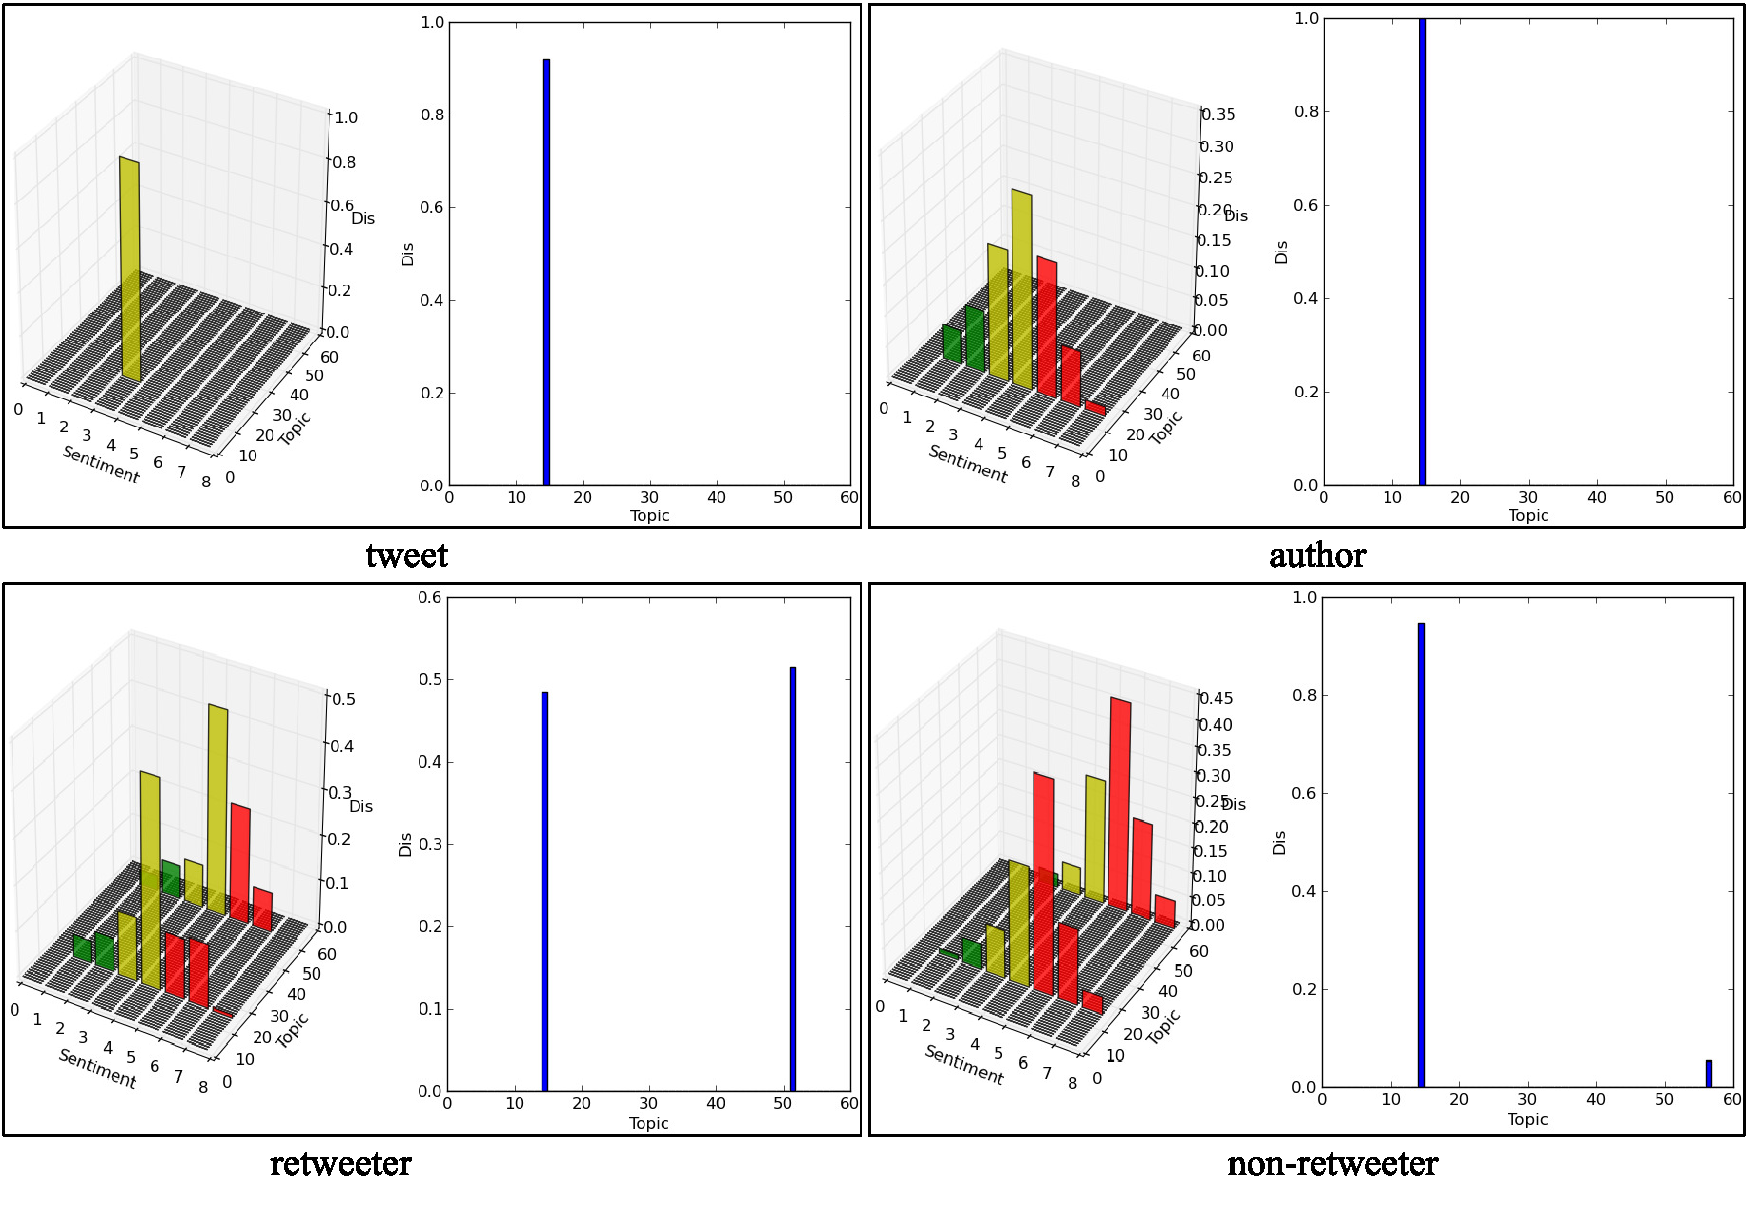
\includegraphics[width=4.5in,height=2.5in]{6-2.pdf}
\caption{An illustration of subjectivity models of a tweet, author and two followers.}
\label{fig5}
\end{figure}

It is obvious that the tweet is about the $ 14^{th} $ topic, and the opinion is neutral.
The author concentrates on the $ 14^{th} $ topic, and his opinion is mainly neutral.
% ($O_{u_{a}}^{14} =( 0, 0.04, 0.05, 0.25, 0.35, 0.25, 0.05,  0.01 )$). 
As for two followers, the retweeter has tweeted on two topics (the $ 14^{th} $ and $ 52^{nd} $ topic) uniformly 
%(with $ w_{u_{r}}(14)=0.48 $) 
and his opinion on the $ 14^{th} $ topic is mainly neutral.
%($O_{u_{r}}^{14} =( 0, 0.02, 0.04, 0.15, 0.50, 0.13,  0.15,  0.01)$). 
While the non-retweeter has also talked about two topics ($ 14^{th} $ and $ 56^{th} $ topic), but he is mainly interested in the $ 14^{th} $ topic 
%(with $ w_{u_{n}}(14)=0.98 $) 
and his opinion is positive.
% ($O_{u_{n}}^{14} =( 0, 0.01, 0.04, 0.10, 0.25, 0.45, 0.13, 0.02)$).

Table~\ref{tab4} shows the three subjectivity similarities for both retweeter and non-retweeter. It is clear that except for the similarity between the tweet and its author, the other two subjectivity similarities of the retweeter are much larger than the non-retweeter.
\begin{table}[h]
\scriptsize
\centering
\caption{ Illustration of example subjectivity similarities}
\label{tab4}
\begin{tabular}{|c|c|c|c|}
\hline
Similarity & $ Sim(f,t) $ & $ Sim(f,u_a)  $ & $ Sim(u_a,t)  $\\
\hline
Retweeter & 0.854 & 0.967 & 0.886\\
\hline
Non-retweeter & 0.805 & 0.919 & 0.886\\
\hline
\end{tabular}
\end{table} 
They have common interest (the $ 14^{th} $ topic), and furthermore the non-retweeter is more similar with the tweet and its author than the retweeter in terms of topics. But their different opinions towards the topic elicit their different behaviors, which verifies our model can help better understanding the retweeting behavior not only from topics but also opinions.

\subsection{Performance Evaluation}

We carried out the retweeting prediction experiments in three stages. Firstly we compared our model against other topic-based models including TF-IDF model (modeling user interests using bag-of-words), entity-based model (using entities extracted from the UGC) and hashtag-based model (using hashtags used in the UGC)\upcite{abel2011analyzing}.
Secondly, our model was compared with two generative topic-sentiment models (TSM model\upcite{mei2007topic} and JST model\upcite{lin2009joint}). TSM and JST can also model topic and topic related sentiment simultaneously. We also use Equation~\ref{subsim} to calculate three  subjectivity similarities for bith TSM and JST as our method in section~\ref{retweet}, and combine them together in the predction.

The subjectivity model has been proposed to catch the subjective motivation of users based on UGC, whereas other important factors associated with retweeting behavior are not considered, such as network topology and meta-data of users. 
Therefore, our model is also compared with the method of Luo \emph{et al.}~\upcite{Luo:2013RMF}(marked as ``LUO''), in which different factors that might affect rewteeting behaviors are considered.
They only use bag-of-words to model user interests, so we also carried out combining experiments to demonstrate that the performance of prediction can be improved by replacing their bag-of-words model with our model (marks with ``LUO+'' prefix). 
\begin{table}[htb]
\scriptsize
\centering
\caption{Accuracy performance. A significant improvement over baseline with $ \ast $ and LUO's model with $ \ddagger $ ($p < 0.05$).}
\label{tab3}
\begin{tabular}{|l|l|l|l|}
\hline
Feature & Accuracy(\%) & Feature & Accuracy(\%)\\
\hline
baseline & 60.85 & & \\
\hline
TF-IDF & 62.85   $\ast$ & LUO & 71.76 $ \ast  $\\
entity & 68.76  $\ast$ & LUO+entity & 72.15 $\ast$\\
hashtag & 59.12  & LUO+hashtag & 68.44 $\ast$\\
\hline
TSM & 67.44 $\ast$ & LUO+TSM & 68.23 $\ast$\\
JST & 68.13 $\ast$ & LUO+JST & 70.53 $\ast$\\
\hline
$ Sim(f,t) $ & 73.88   $\ast  \quad \ddagger $ &LUO+$ Sim(f,t)$ & 74.04  $ \ast \quad \ddagger $\\
$ Sim(f,u_a)  $ & 70.04   $\ast  $ & LUO+$ Sim(f,u_a)$ & 70.27  $ \ast $\\
$ Sim(u_a,t)  $ & 69.64   $\ast  $ & LUO+$ Sim(u_a,t)$ & 71.86  $ \ast $\\
$ sim_{all}  $ & \textbf{75.64}   $\ast \quad \ddagger $ & LUO+$ sim_{all}  $ & \textbf{78.15}  $ \ast \quad \ddagger $\\
\hline
\end{tabular}
\end{table}

The logistic regression classifier is used for training and testing in a 5-fold cross-validation manner.
We set a baseline, which simply predicts users who have retweeted the author previously as the retweeters of target tweet. 
All results are presented in Table~\ref{tab3} in terms of accuracy.

Firstly, all models except the hashtag-based model outperform the baseline (60.85\%) significantly. While for hashtag-based model, the accuracy is only 59.12\%, the reason lies in the sparcity of hashtag in tweets. 

Secondly, $ Sim(f,t) $ and $ sim_{all}  $ outperform ``LUO'' (71.76\%) significantly.
The best performance is achieved by the $ sim_{all}  $ (75.64\%), for which we add three similarities to the classifier to test the impact of their combination. 
The performance of TF-IDF model (62.85\%) is a little better than baseline. 
The entity-based model (68.76\%) is very close to  $ Sim(f,u_a)$ (70.04\%) and $ Sim(u_a,t)  $ (69.64\%), and the difference is not significant.

Thirdly, the performance of two topic-sentiment models (TSM: 67.44\%, JST: 68.13\%) is not as good as our models. The reason lies in that they use a binary sentiment representation (positive or negative), which can not differentiate opinions elaborately. Our model can capture more subtle and fine-grain sentiment, which could distinguish different subective motivation of retweeting behavior.

Finally, in the combining evaluation, $ Sim(f,t) $ gives a significant improvement (LUO+$ Sim(f,t) $, 2.12\% improvement) over ``LUO'', but other two similarities and the entity-based model can not improve performance significantly. The performance is even degraded after combining with the hashtag-based model and two topic-sentiment models. 
But noticing that, the most significant improvement(LUO+$ sim_{all}  $, 6.39\% improvement) is achieved by combining with all three similarities. 

Above all, the results show that our model can better help predicting retweeting behavior and can be regarded as a useful way to analyze the retweeting behaviors of users. 

\section{Conclusion}
Motivated by the psychological research, this paper postulates that the diffusion behaviors of social media users are affected by their subjectivity. Therefore, a general subjectivity model has been proposed and an efficient framework has been designed to establish the subjectivity model. Also a novel method is proposed to measure the subjectivity similarity. The subjectivity model has been applied to the retweeting analysis considering the attractiveness, sociality and popularity factors, which are quantified with subjectivity similarities. 
Experiment results demonstrate the effectiveness of the proposed model in the retweeting analysis problem and show that the model is able to reach better understanding of retweeting behavior. 
In the future, we will apply our model to other social network analysis task such as link prediction and recommendation. 

